%%%%%%%%%%%%%%%%%%%%%%%%%%%%%%%%%%%%%%%%%
% Jacobs Landscape Poster
% LaTeX Template
% Version 1.0 (29/03/13)
%
% Created by:
% Computational Physics and Biophysics Group, Jacobs University
% https://teamwork.jacobs-university.de:8443/confluence/display/CoPandBiG/LaTeX+Poster
% 
% Further modified by:
% Nathaniel Johnston (nathaniel@njohnston.ca)
%
% This template has been downloaded from:
% http://www.LaTeXTemplates.com
%
% License:
% CC BY-NC-SA 3.0 (http://creativecommons.org/licenses/by-nc-sa/3.0/)
%
%%%%%%%%%%%%%%%%%%%%%%%%%%%%%%%%%%%%%%%%%

%----------------------------------------------------------------------------------------
%	PACKAGES AND OTHER DOCUMENT CONFIGURATIONS
%----------------------------------------------------------------------------------------

\documentclass[final]{beamer}

\usepackage[scale=1.24]{beamerposter} % Use the beamerposter package for laying out the poster

\usetheme{confposter} % Use the confposter theme supplied with this template

\setbeamercolor{block title}{fg=ngreen,bg=white} % Colors of the block titles
\setbeamercolor{block body}{fg=black,bg=white} % Colors of the body of blocks
\setbeamercolor{block alerted title}{fg=white,bg=dblue!70} % Colors of the highlighted block titles
\setbeamercolor{block alerted body}{fg=black,bg=dblue!10} % Colors of the body of highlighted blocks
% Many more colors are available for use in beamerthemeconfposter.sty

%-----------------------------------------------------------
% Define the column widths and overall poster size
% To set effective sepwid, onecolwid and twocolwid values, first choose how many columns you want and how much separation you want between columns
% In this template, the separation width chosen is 0.024 of the paper width and a 4-column layout
% onecolwid should therefore be (1-(# of columns+1)*sepwid)/# of columns e.g. (1-(4+1)*0.024)/4 = 0.22
% Set twocolwid to be (2*onecolwid)+sepwid = 0.464
% Set threecolwid to be (3*onecolwid)+2*sepwid = 0.708

\newlength{\sepwid}
\newlength{\onecolwid}
\newlength{\twocolwid}
\newlength{\threecolwid}
\setlength{\paperwidth}{48in} % A0 width: 46.8in
\setlength{\paperheight}{36in} % A0 height: 33.1in
\setlength{\sepwid}{0.024\paperwidth} % Separation width (white space) between columns
\setlength{\onecolwid}{0.22\paperwidth} % Width of one column
\setlength{\twocolwid}{0.464\paperwidth} % Width of two columns
\setlength{\threecolwid}{0.708\paperwidth} % Width of three columns
\setlength{\topmargin}{-0.5in} % Reduce the top margin size
%-----------------------------------------------------------

\usepackage{graphicx}  % Required for including images
\usepackage{booktabs} % Top and bottom rules for tables

%multi-row
\usepackage{multirow}
 

%----------------------------------------------------------------------------------------
%	TITLE SECTION 
%----------------------------------------------------------------------------------------

\title{CS230 - Learning Minichess Without Human Knowledge} % Poster title

\author{Karthik selvakumar Bhuvaneswaran} % Author(s)

\institute{karthik0@stanford.edu} % Institution(s)

%----------------------------------------------------------------------------------------

\begin{document}

\addtobeamertemplate{block end}{}{\vspace*{2ex}} % White space under blocks
\addtobeamertemplate{block alerted end}{}{\vspace*{2ex}} % White space under highlighted (alert) blocks

\setlength{\belowcaptionskip}{2ex} % White space under figures
\setlength\belowdisplayshortskip{2ex} % White space under equations

\begin{frame}[t] % The whole poster is enclosed in one beamer frame

\begin{columns}[t] % The whole poster consists of three major columns, the second of which is split into two columns twice - the [t] option aligns each column's content to the top

\begin{column}{\sepwid}\end{column} % Empty spacer column

\begin{column}{\onecolwid} % The first column

\setbeamercolor{block alerted title}{fg=black,bg=ngreen} % Change the alert block title colors
\setbeamercolor{block alerted body}{fg=black,bg=white} % Change the alert block body colors
%----------------------------------------------------------------------------------------
%	OBJECTIVES
%----------------------------------------------------------------------------------------

\begin{alertblock}{Abstract}

Using WebRTC we are trying to develop a product called 'Ping' used for audio, mult-video, file and screen sharing.
\begin{itemize}
\item Ping uses WebRTC for the source of data exchange and XMPP Server for signalling and transporting.
\item Ping works on Browser to Browser connections instead of naive client server approach.
\item Ping guarentees high scalability and upto 60\% more efficiency than existing systems.
\end{itemize}

\end{alertblock}

%----------------------------------------------------------------------------------------
%	INTRODUCTION
%----------------------------------------------------------------------------------------

\begin{block}{Logic and MCTS}

\begin{itemize}
\item WebRTC is an upcoming standard that aims to improve real time communication among web browsers in peer to peer fashion.
\item Ping uses WebRTC which allows browsers to natively support interactive peer to peer communication and realtime collaboration.
\end{itemize}

\begin{figure}
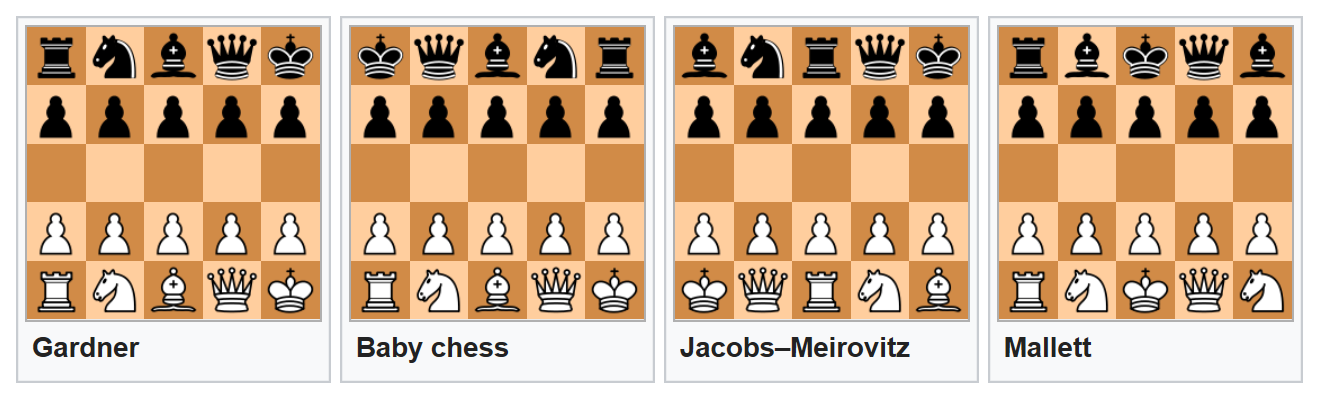
\includegraphics[width=1.0\linewidth]{minichess.png}
\caption{Popular Minichess Board Layouts}
\end{figure}


\[ l = \sum (v_{\theta}(s_{t}) - z_{t})^{2}+ \vec{\pi_{t}} log(\vec{p_{\theta}}(s_{t}))  \]


\end{block}

%------------------------------------------------

%----------------------------------------------------------------------------------------

\end{column} % End of the first column

\begin{column}{\sepwid}\end{column} % Empty spacer column

\begin{column}{\twocolwid} % Begin a column which is two columns wide (column 2)

\begin{columns}[t,totalwidth=\twocolwid] % Split up the two columns wide column

\begin{column}{\onecolwid}\vspace{-.6in} % The first column within column 2 (column 2.1)

%----------------------------------------------------------------------------------------
%	MATERIALS
%----------------------------------------------------------------------------------------

\begin{block}{Distributed Architecture}

We designed an efficient architecture for Ping to withstand high traffic.

\begin{itemize}
\item At start browsers do not know each other.
\item WebRTC mediates the setup process through the XMPP server of Ping.
\end{itemize}

\begin{figure}
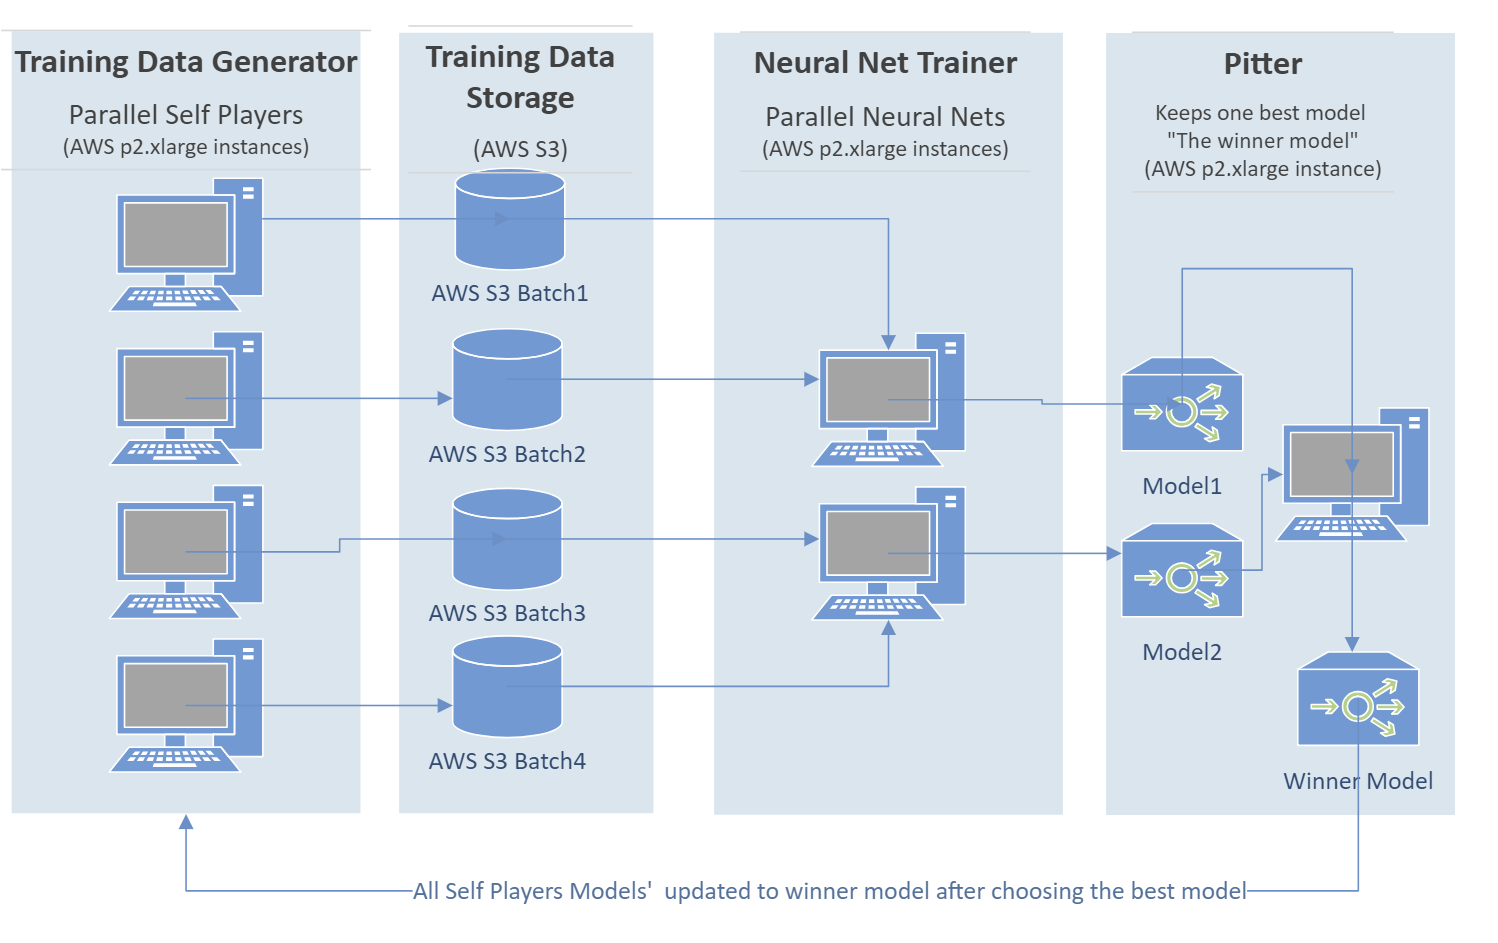
\includegraphics[width=1.0\linewidth]{distributed_arch.png}
\caption{Distributed Cloud Architecture for Reinforcement Learning}
\end{figure}


\end{block}

%----------------------------------------------------------------------------------------

\end{column} % End of column 2.1

\begin{column}{\onecolwid}\vspace{-.6in} % The second column within column 2 (column 2.2)

%----------------------------------------------------------------------------------------
%	METHODS
%----------------------------------------------------------------------------------------

\begin{block}{Performance Gain Distributed vs Single Instance}
\begin{figure}
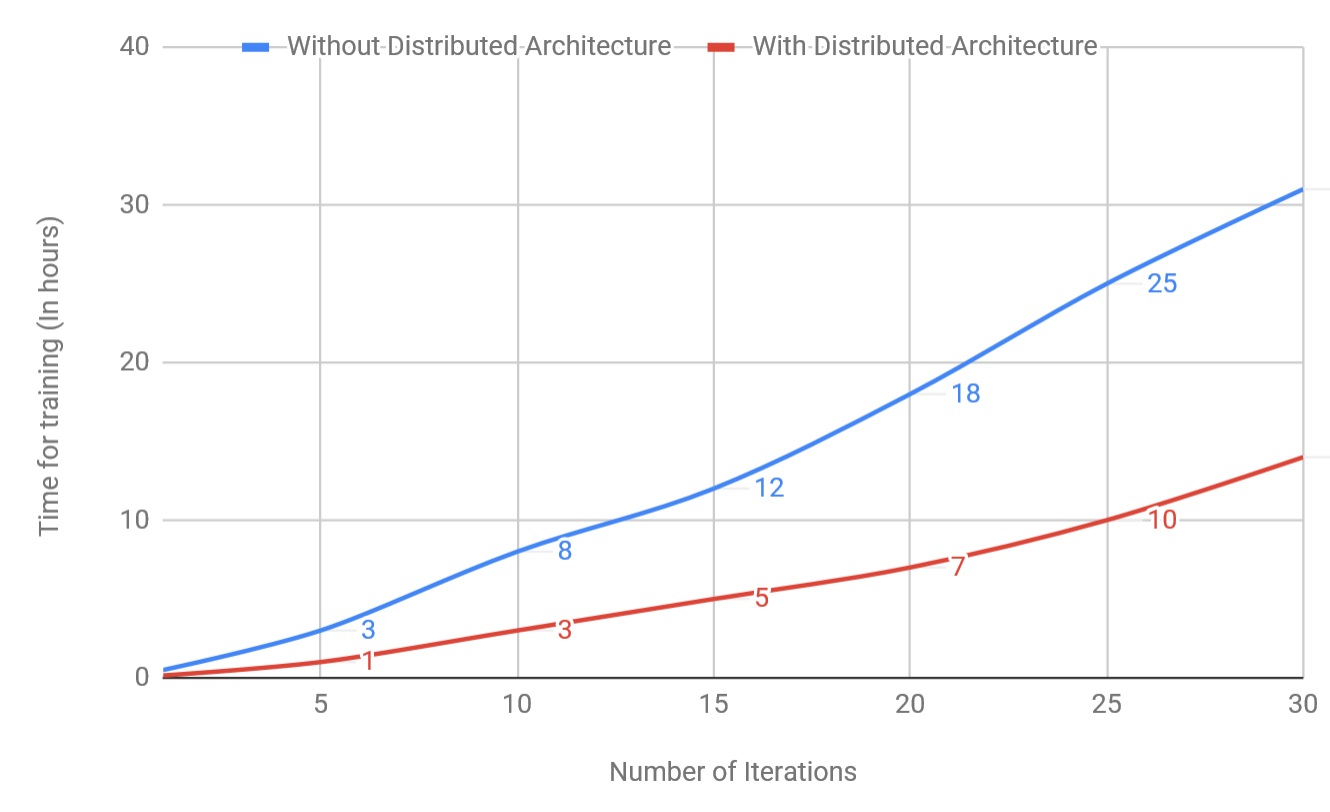
\includegraphics[width=1.0\linewidth]{performance_gain.png}
\caption{Distributed Cloud Architecture for Reinforcement Learning}
\end{figure}


\end{block}

%----------------------------------------------------------------------------------------

\end{column} % End of column 2.2

\end{columns} % End of the split of column 2 - any content after this will now take up 2 columns width

%----------------------------------------------------------------------------------------
%	IMPORTANT RESULT
%----------------------------------------------------------------------------------------



%----------------------------------------------------------------------------------------

\begin{columns}[t,totalwidth=\twocolwid] % Split up the two columns wide column again

\begin{column}{\onecolwid} % The first column within column 2 (column 2.1)

%----------------------------------------------------------------------------------------
%	MATHEMATICAL SECTION
%----------------------------------------------------------------------------------------

\begin{block}{Neural Network and hyperparams}

\begin{itemize}
\item RTC Peer connection is the WebRTC API that handles stable and efficient communication of streaming data between peers.
\end{itemize}


\begin{figure}
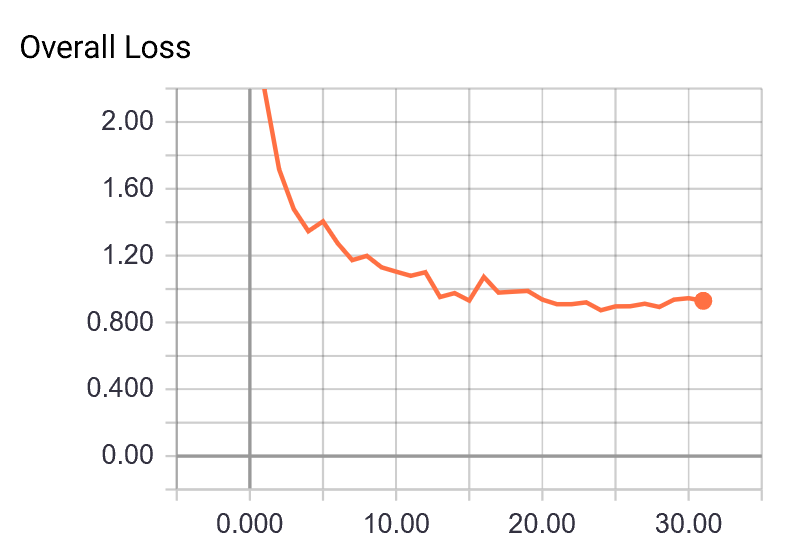
\includegraphics[width=0.3\linewidth]{overall_loss.png}
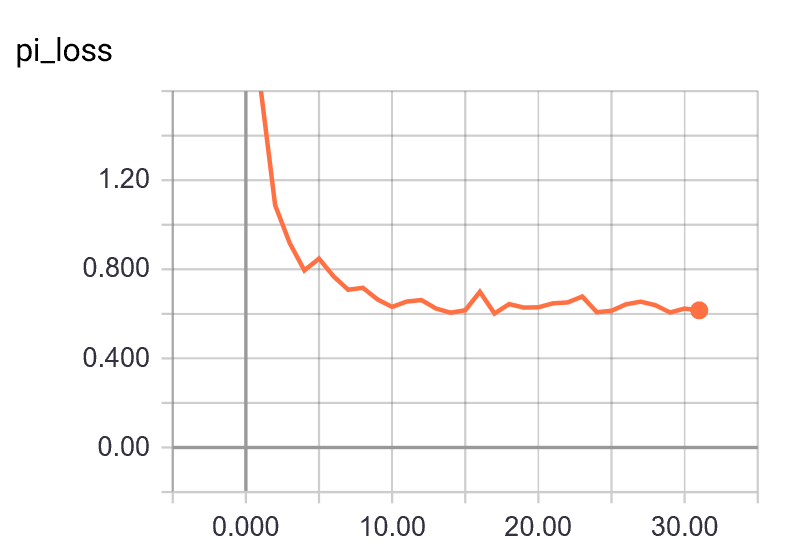
\includegraphics[width=0.3\linewidth]{pi_loss.png}
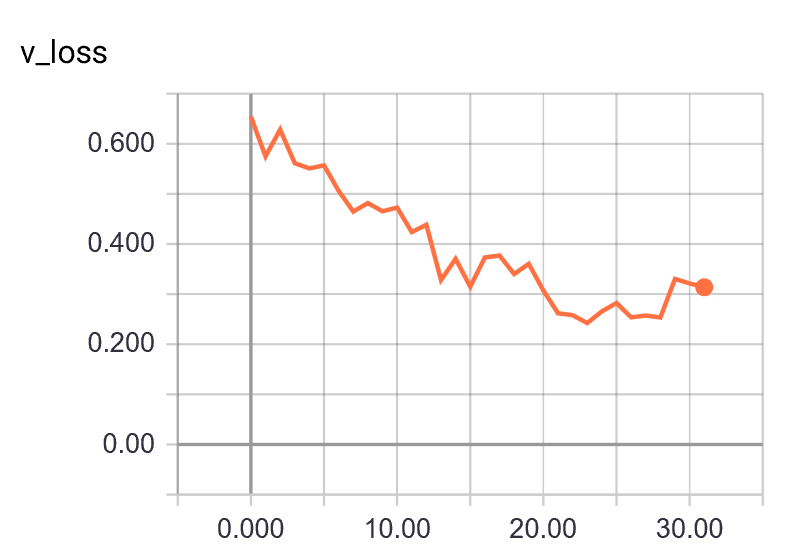
\includegraphics[width=0.3\linewidth]{value_loss.png}
\caption{Loss values after each epoch}
\end{figure}


\begin{figure}
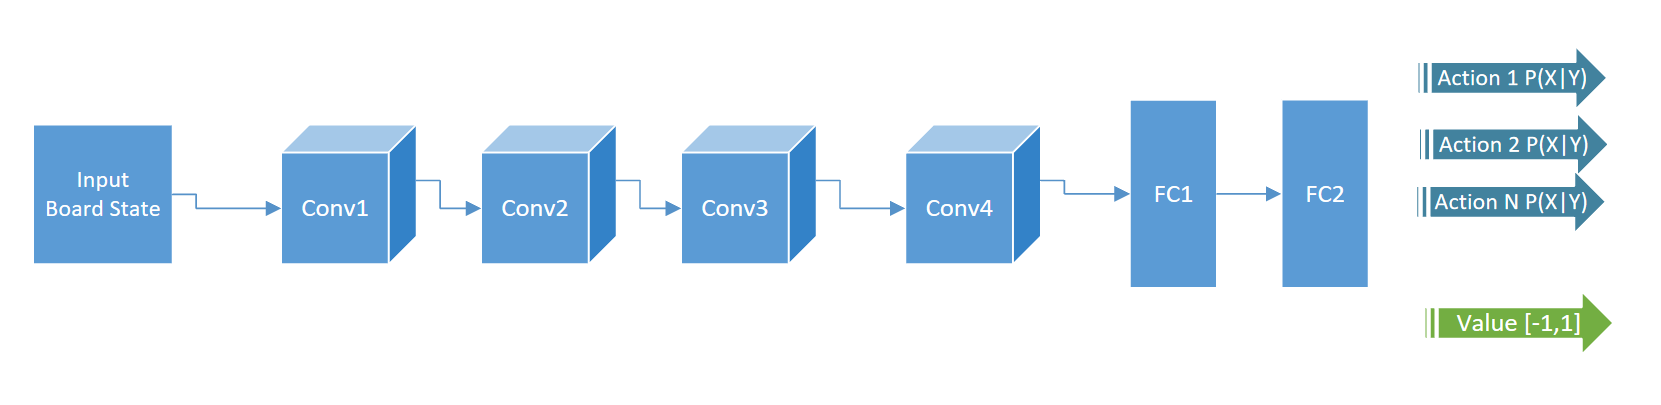
\includegraphics[width=0.8\linewidth]{cnn.png}
\caption{Baseline Random vs Greedy vs Neural Net}
\end{figure}

\end{block}

%----------------------------------------------------------------------------------------

\end{column} % End of column 2.1

\begin{column}{\onecolwid} % The second column within column 2 (column 2.2)

%----------------------------------------------------------------------------------------
%	RESULTS
%----------------------------------------------------------------------------------------

\begin{block}{Baseline Random vs Greedy vs Neural Net}


\begin{figure}
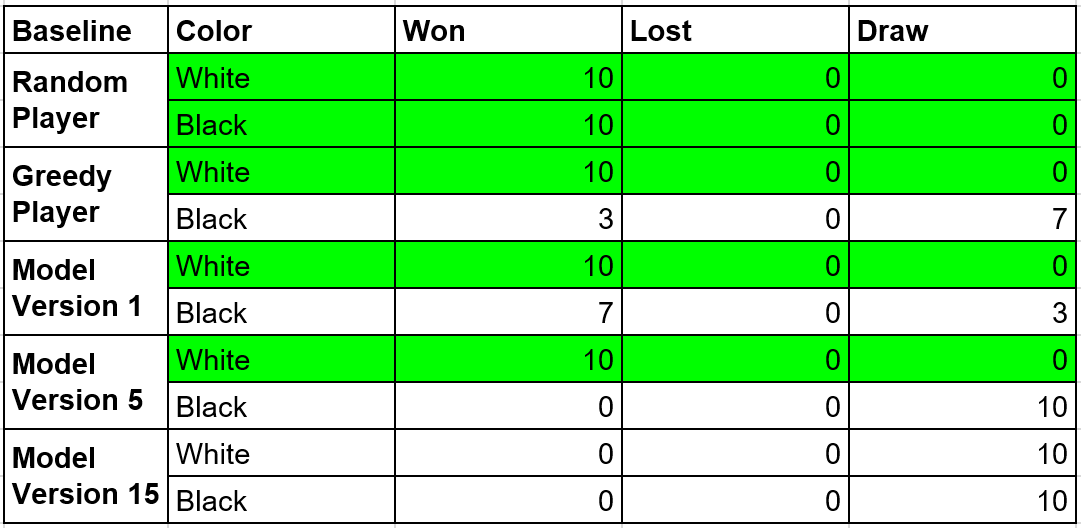
\includegraphics[width=0.8\linewidth]{baseline.png}
\caption{Baseline Random vs Greedy vs Neural Net}
\end{figure}

\begin{figure}
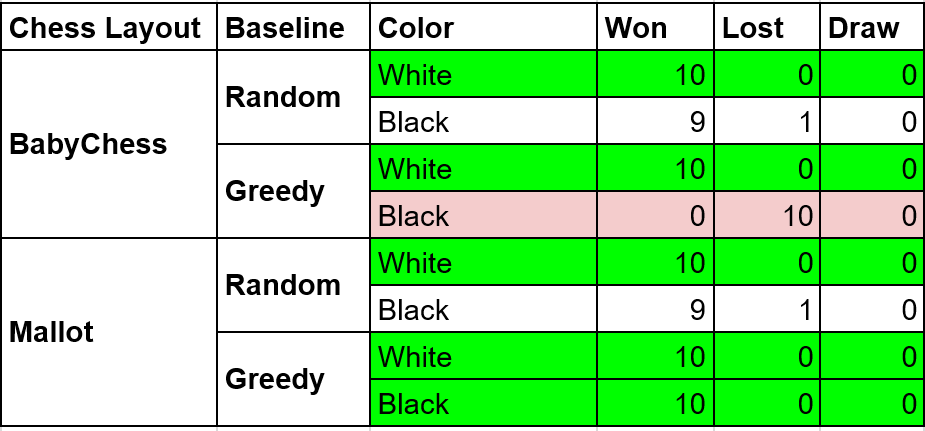
\includegraphics[width=0.8\linewidth]{diff_layouts.png}
\caption{Best Model on directly used on different layouts}
\end{figure}

\end{block}

%----------------------------------------------------------------------------------------

\end{column} % End of column 2.2

\end{columns} % End of the split of column 2

\end{column} % End of the second column

\begin{column}{\sepwid}\end{column} % Empty spacer column

\begin{column}{\onecolwid} % The third column


%----------------------------------------------------------------------------------------
%	CONCLUSION
%----------------------------------------------------------------------------------------

\begin{block}{Iteration to Reach the performance}

\begin{itemize}
\item Though there are existing systems like Skype and Hangouts, Ping guarentees around 60\% more efficiency.
\item Ping also guarentees high scalability. Around 3000 users per second.
\item As WebRTC is leveraging communication, Ping uses WebRTC to improved end user experience.
\end{itemize}

\end{block}

\begin{block}{Interesting Moves and Neural Net values}

\begin{itemize}
\item Though there are existing systems like Skype and Hangouts, Ping guarentees around 60\% more efficiency.
\end{itemize}

\end{block}


\begin{block}{Conclusion}

\begin{itemize}
\item Though there are existing systems like Skype and Hangouts, Ping guarentees around 60\% more efficiency.
\item Ping also guarentees high scalability. Around 3000 users per second.
\end{itemize}

\end{block}

%----------------------------------------------------------------------------------------
%	ADDITIONAL INFORMATION
%----------------------------------------------------------------------------------------



%----------------------------------------------------------------------------------------
%	REFERENCES
%----------------------------------------------------------------------------------------

\begin{block}{References}


\begin{itemize}{}

\item Gardner's Minichess Variant is solved. Mehdi Mhalla et al. {\em arXiv e-print (arXiv:1307.7118) }
\item Learning to Play Othello Without Human Knowledge Surag Nair et al {\em github.com/suragnair/alpha-zero-general}
\item Mastering Chess and Shogi by Self-Play with a General Reinforcement Learning Algorithm. Silver et al. 2017a
\end{itemize}

\end{block}

%----------------------------------------------------------------------------------------
%	ACKNOWLEDGEMENTS
%----------------------------------------------------------------------------------------



%----------------------------------------------------------------------------------------
%	CONTACT INFORMATION
%----------------------------------------------------------------------------------------


\begin{alertblock}{Contact Information}

\begin{itemize}
\item Web: \href{https://github.com/karthikselva/alpha-zero-general/tree/minichess}{https://github.com/karthikselva/alpha-zero-general/tree/minichess}
\item Email: karthik0@stanford.edu
\end{itemize}

\end{alertblock}


%----------------------------------------------------------------------------------------

\end{column} % End of the third column

\end{columns} % End of all the columns in the poster

\end{frame} % End of the enclosing frame

\end{document}
